\chapter{Geophysics}\label{ch:equations}

This chapter introduces geophysics as a way of thinking about the Earth using physical principles, mathematical models, and quantitative reasoning. Rather than attempting to reproduce geological complexity in detail, geophysics abstracts the Earth into fields, material properties, and governing equations. This abstraction allows us to infer otherwise inaccessible aspects of the Earth—from lithospheric structure and mantle dynamics to groundwater flow, natural hazards, and resource distribution.

The goal of this chapter is to establish a shared conceptual framework that will be used throughout the book. We begin by defining what geophysics is and what it seeks to accomplish. We then introduce the idea of fields and their relationship to material properties, discuss why smooth mathematical descriptions are used to model a discontinuous Earth, and explain why equations and simplified models are essential tools rather than optional conveniences. We conclude with a discussion of how this conceptual framework supports both classical and modern geophysical practice and how it connects to the chapters that follow.

\section{What is Geophysics?}
I'll give two answers the above question, one which you probably suspect.  Firstly, geophysics applies the principles of physics to the study of the Earth and other planetary bodies.  Geophysics is used to probe the structure, composition, physical state, and processes acting with the Earth's interior.  We employ the principles of physics to explore for resources and energy, to monitor the environment and climate, identify and monitor natural hazards, investigate archaeological sites, search for unexploded ordinance, and probe the inner workings of the Earth.

Second, geophysics uses classical physics to model the past, present and future physical state of the Earth---Earth's geological evolution.  Often the Earth can be reduced to a simple process or set of simple processes acting in concert that allow one to identify the key physical processes and properties driving that change.  Through simple models we can see how changes in these key parameters may alter the observed behavior.

It is not possible to cover all of geophysics in one course.  Entire books are written about each of the subdisciplines discussed in these notes.  This course represents a survey of a selected few topics that find applications in industrial and academic settings.  Many of the examples I will use are academic in nature and may, at times, seem far removed from physical reality, but I assure you that the principles and concepts are directly applicable to the real world.

\section{Observation, Abstraction, and Earth Models}

In geophysics, we rarely observe the Earth directly. Instead, we measure physical fields at discrete locations—gravity, magnetic field, temperature, voltage, pressure, or ground motion—and infer the distribution of material properties that produced them. Nearly everything in this book is concerned with relating fields to properties.

Geophysical measurements are indirect, incomplete, and affected by uncertainty. Earth models therefore serve as abstractions that connect observations to physical interpretation. These models are not expected to reproduce the full geological complexity of the Earth but instead to capture the dominant physical processes responsible for the observed data.

\section{Fields}

What is a field?  Each point in space and time may be defined by a set of functions, a {\it field}.  There are three basic types of fields scalars, vectors and tensors.

\emph{Scalar fields} are described by a single function in space and time.  Each point in space has a single magnitude (e.g., density, temperature, pressure).

\emph{Vector fields} are defined by three functions in space and time.  Each point in space has a single magnitude and a direction (e.g., velocity, force, electric field).

\emph{Tensor fields} are technically generalizations of scalar and vector fields, but can be higher order.  Each point in space may be defined by a multiple magnitudes and directions.  While vector fields can be represented by an arrow at each point in space with a length equal to the magnitude and the orientation defining the direction, tensors may be defined by multiple arrows and directions that can be visualized as an ellipse or an ellipsoid at each point in space (e.g., stress, strain, electrical impedance).

Fields can also relate to material properties (e.g., density, magnetization, seismic velocity, resistivity), describe the system states (e.g., temperature, pressure), or force fields that act on each point in space and have the potential to do work (e.g., gravitational attraction, heat flow, strain rate).

Something else that will arise from time to time will be {\it field lines}, which are sometimes refered to as {\it flow lines} depending upon the application. Field lines represent the direction a partical would travel going in the direction of highest magnitude, force, or potential to lowest.  We draw field lines with arrows and they may be open (the ends do not meet) or closed (the ends join).  Although, depending upon the convention, we sometimes draw the arrows in the opposite direction.

In contrast, {\it isolines} trace out a continuous set of points at constant potential, force, or magnitude and are orthogonal ($\perp$) to the field lines at all times.  A common example is contour lines on a topographic map which trace lines of constant elevation.  A rain drop falling on topography would head in the direction of the flow lines.  We can define also define an isosurface or equipotential surface that defines a surface of constant magnitude and can be open like a sheet or closed like a balloon (enclosing a region of space).

\subsection{Continuity and Differentiability}

\emph{The Earth is piecewise discontinuous, but the equations we use assume smoothness.}

Many of the mathematical tools used in geophysics rely on assumptions of continuity and differentiability. These assumptions are often introduced as mathematical requirements, but they also have clear physical interpretations and limitations when applied to the Earth.

The Earth is not a smooth object. Changes in lithology, phase, composition, and structure can produce abrupt changes in material properties such as density, thermal conductivity, elastic moduli, or seismic velocity. As a result, these properties are often discontinuous functions of position.

In contrast, the physical fields we seek to model—such as temperature, gravitational potential, pressure, or displacement—are generally continuous across material boundaries. For example, temperature does not jump abruptly at a lithologic contact, even though the thermal conductivity may. However, the spatial derivatives of these fields need not be continuous. A sharp change in material properties often produces a kink in the field, corresponding to a discontinuity in its gradient.

Most governing equations in geophysics are formulated under the assumption that the relevant fields are continuous and differentiable. These assumptions are required to define derivatives and apply differential operators. When the Earth violates these assumptions, we must either restrict our analysis to regions where the assumptions hold or reformulate the problem in a way that preserves the underlying physical principles, such as conservation of flux.

This distinction between discontinuous properties and continuous fields is central to geophysical modeling. It explains why material interfaces require special treatment, why numerical methods must be designed carefully near sharp contrasts, and why many models enforce smoothness even when the Earth itself is not smooth.

Throughout this book, we will make explicit when continuity and differentiability are assumed, why those assumptions are reasonable, and how their limitations influence both analytic and numerical solutions.  Several of the techniques introduced later in this book can be understood as different ways of managing the tension between a discontinuous Earth and smooth mathematical descriptions.

\section{Geophysical Equations}

There are many partial differential equations (PDEs) but only a handful are commonly used in geophysics.  We will only cover three equations: the potential field equation (Laplace's---or more generally Poisson's equations), the diffusion equation, and the wave equation.  We will study a wide range of physical applications.  Many of these applications are governed by the same or similar equations, differing only by the physical properties that create geophysical fields.

\subsection{Physical Laws and Constitutive Relations}

Governing equations describe the structure of geophysical processes, but they do not by themselves specify how the Earth responds. That information enters through constitutive relations, which link fields such as stress, flux, or current to material properties. These relations determine how forces are transmitted, how energy is transported, and how variations in Earth structure are expressed in observable fields (Chapters~\ref{ch:potential}--\ref{ch:waves}).

Material properties such as density, elastic moduli, electrical conductivity, and thermal diffusivity vary spatially and reflect geological composition, temperature, pressure, and fabric. In this sense, constitutive relations provide the primary connection between abstract equations and the physical Earth. Through these relations, physical properties control how the Earth responds to forcing and how different regions contribute to measured signals. Chapter~\ref{ch:physprop} examines these properties and how they are defined and related to geological materials, providing the link between governing equations and real Earth structure.

Although the governing equations recur across many subdisciplines, differences in material properties and constitutive behavior lead to very different observable phenomena. The essential point here is that geophysical equations acquire physical meaning only when paired with appropriate constitutive relations and property models.

\subsection{Potential Fields} \label{sec:laplace}

No time dependence.

Laplace's and Poisson's equations belong to a special class of partial differential equations called elliptical equations (Chapter~\ref{ch:potential}).  Elliptic equations describe fields that respond instantly to sources (steady-state); parabolic equations describe processes that spread with time (diffiusion); hyperbolic equations describe signals that propagate at finite speed (wave propagation).  These elliptical potential fields equations are defined as
\begin{align}
    \coreeq
    \laplacian u &= 0 & \text{Laplace's equation}, \\
    \coreeq
    \laplacian u &= s & \text{Poisson's equation},
\end{align}
where $u(x,y,z)$ is a scalar potential.  We use Laplace's equation when we are outside of the source region and Poisson's equation within the source region.  A source region is within the body that creates the potential field.  In geophysics, we use these equations to describe gravity, magnetics, voltage, temperature; although the fields must be steady-state (no temporal variation) in order to apply these equations. Poisson's relationship for several geophysical potentials are listed below:
\begin{table}[h!]
    \centering
    \caption{Common uses of the potential fields (elliptical) equation in geophysics.}
    \label{tab:pfeq}
    \begin{tabular}{lcc}
        \toprule
        \textbf{Poisson's Equation} &
        \textbf{Field} &
        \textbf{Chapter} \\
        \midrule
        $\laplacian U = 4 \pi G \rho_m$ & gravity & Ch.~\ref{ch:gravity} \\
        $\laplacian A = -\mu \div \vb{M}$ & magnetics & Ch.~\ref{ch:magnetics} \\
        $\laplacian T = -\frac{A}{k}$ & thermal & Ch.~\ref{ch:geothermics1} \\
        $\laplacian V = -\frac{\rho_e}{\epsilon}$ & electrical & Ch.~\ref{ch:electrostatics}\\
        \bottomrule
    \end{tabular}
\end{table}
While not exactly the same, they are remarkably similar in each case.

\ntextbox{Vector Operators}{
    \begin{center}
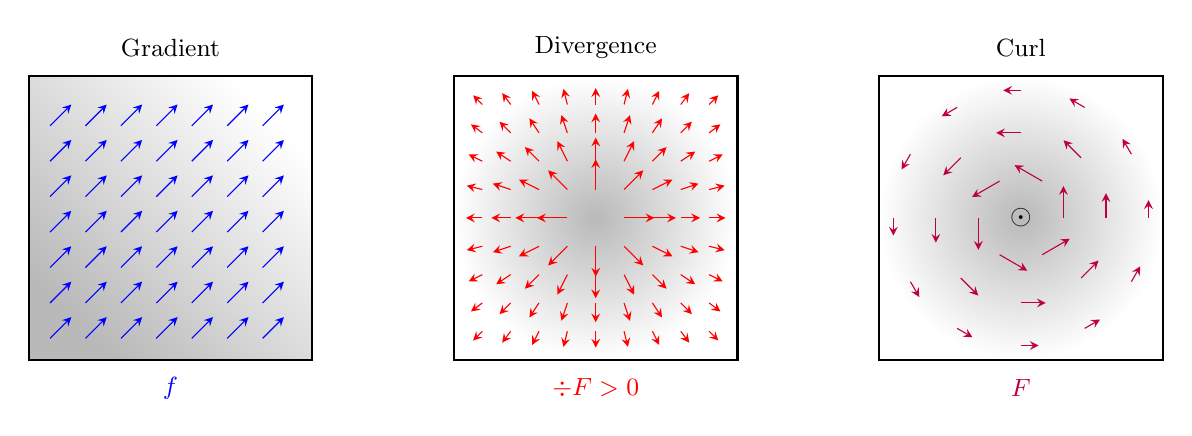
\begin{tikzpicture}[scale=0.9,>=stealth] 
    % Gradient panel 
    \begin{scope} 
        \shade[
            shading=axis,
            left color=gray!55,
            right color=white,
            shading angle=135
        ] (-2,-2) rectangle (2,2);
        \draw[thick] (-2,-2) rectangle (2,2);
        \node at (0,2.4) {\small Gradient};
        \foreach \x in {-1.7,-1.2,...,1.5} 
            \foreach \y in {-1.7,-1.2,...,1.5}
                \draw[->,blue] (\x,\y) -- +(0.3,0.3);
        \node[blue] at (0,-2.4) {\small $\grad{f}$}; 
    \end{scope}

    \begin{scope}[xshift=6cm]
        \shade[
            inner color=gray!55,
            outer color=white,
        ] (-2,-2) rectangle (2,2);
        \draw[thick] (-2,-2) rectangle (2,2);
        \node at (0,2.4) {\small Divergence};

        % Vector field
        \foreach \x in {-1.6,-1.2,...,1.7} {
            \foreach \y in {-1.6,-1.2,...,1.7} {

                % radius
                \pgfmathsetmacro{\r}{sqrt(\x*\x + \y*\y)}

                % avoid division by zero at center
                \ifdim \r pt > 0.05pt

                    % unit vector scaled by decaying function
                    \pgfmathsetmacro{\scale}{0.6/(1 + \r)}

                    \draw[->,red]
                        (\x,\y) --
                        ({\x + \scale*\x/\r}, {\y + \scale*\y/\r});

                \fi
            }
        }

        \node[red] at (0,-2.4) {\small $ \div{\vb{F}} > 0$};
    \end{scope}

    % Curl panel
    \begin{scope}[xshift=12cm]
        \shade[
            inner color=gray!55,
            outer color=white,
        ] (-2,-2) rectangle (2,2);
        \draw[thick] (-2,-2) rectangle (2,2);

        \node at (0,0) {$\odot$};

        \node at (0,2.4) {\small Curl};

        % Inner ring of circulation
        \foreach \a in {0,60,...,330}
            \draw[->,purple] (\a:0.6) -- +(\a+90:0.45);

        \foreach \a in {0,45,...,330}
            \draw[->,purple] (\a:1.2) -- +(\a+90:0.35);

        % Outer ring of circulation
        \foreach \a in {0,30,...,330}
            \draw[->,purple] (\a:1.8) -- +(\a+90:0.25);

        \node[purple] at (0,-2.4) {\small $\curl{\vb{F}}$};
    \end{scope}
\end{tikzpicture}
\textbf{Figure~\thefigure:} Visual depictions of a gradient of a scalar fuction (a), divergence of a vector function (b), and the curl of a vector function (c).
\label{fig:del}
\end{center}


    \textbf{Gradient}, $\grad$, is a linear operator that tells us about the direction of maximum increase (slope) of a field.  Applied to a scalar function, $f$, the gradient is
    \[
        \grad{f} = \pdv{f}{x}\vu{x} + \pdv{f}{y}\vu{y} + \pdv{f}{z}\vu{z}.
    \]
    In geothermics, gradients relate temperature fields to heat flux (e.g., Fourier's law). Physically, the gradient answers the question: \emph{which way is uphill, and how steep is it?}

    We can apply the gradient to a vector field, $\vb{F}$, which results in the Jacobian, a second-order tensor,
    \[
        \grad{\vb{F}} = 
        \begin{bmatrix}
            \pdv{F_x}{x} & \pdv{F_x}{y} & \pdv{F_x}{z} \\[0.4em]
            \pdv{F_y}{x} & \pdv{F_y}{y} & \pdv{F_y}{z} \\[0.4em]
            \pdv{F_z}{x} & \pdv{F_z}{y} & \pdv{F_z}{z} 
        \end{bmatrix} ,
    \]
    and is common in electromagnetics and seismics.

    \medskip \textbf{Divergence}, $\div$, measures the net outward flux of a vector field per unit volume: 
    \[
        \div{\vb{F}} = \pdv{F_x}{x} + \pdv{F_y}{y} + \pdv{F_z}{z} .
    \]
    Positive divergence indicates a source; negative divergence indicates a sink. In the heat equation, divergence expresses conservation of energy by accounting for how heat flows into or out of a volume.

    \medskip \textbf{Curl}, $\curl$, measures the local rotation or circulation of a vector field,
    \[
        \curl{\vb{F}} = 
        \left( \pdv{F_z}{y} - \pdv{F_y}{z} \right) \vu{x} +
        \left( \pdv{F_x}{z} - \pdv{F_z}{x} \right) \vu{y} +
        \left( \pdv{F_y}{x} - \pdv{F_x}{y} \right) \vu{z} .
    \]
    The direction of the curl follows the right-hand rule: pointing your thumb in the direction of the field, your fingers curl in the direction of circulation. Curl is prominent in Maxwell's equations, where it relates time-varying electric and magnetic fields, and it is also central in fluid dynamics through vorticity.

    \medskip \textbf{Laplacian}, $\laplacian = \div \grad$, measures the local curvature of a scalar field,
    \[
        \laplacian f = \pdv[2]{f}{x} + \pdv[2]{f}{y} + \pdv[2]{f}{z} .
    \]
    The Laplacian is features prominantly in the potential, diffusion, and wave equations.
}{mathtool}

\subsection{Diffusion Equation}\label{sec:diffusion}

The diffusion equation belongs to the class of partial differential equations called parabolic equations (Chapter~\ref{ch:diffusion}).  These equations are defined as
\begin{equation}
    \coreeq
    \pdv{u}{t} = D \laplacian u,
\end{equation}
where u(x,y,z) can be either a scalar or vector and $D$ is the diffusion constant.  We can add an additional term to describe motion, making the advection-diffusion equation,
\[
    \pdv{u}{t} = D \laplacian u + \div (V u),
\]
where $V$ is the velocity.

In geoscience, we use the diffusion equation to describe the diffusion of heat and chemical species:
\begin{table}[h!]
    \centering
    \caption{Common uses of the diffusion (parabolic) equation in geophysics.}
    \label{tab:diffusioneq}
    \begin{tabular}{lcc}
        \toprule
        \textbf{Diffusion Equation} &
        \textbf{Field} &
        \textbf{Chapter} \\
        \midrule
        $\pdv{T}{t} = \kappa \laplacian T$ & thermal & Ch.~\ref{ch:geothermics2} \\
        $\pdv{C}{t} = D \laplacian C$ & chemical & --- \\
        $\laplacian \vb{E} = \mu \sigma \pdv{\vb{E}}{t}$ & electrical & Ch.~\ref{ch:EMmethods} \\
        $\laplacian \vb{H} = \mu \sigma \pdv{\vb{H}}{t}$ & magnetic & Ch.~\ref{ch:EMmethods} \\
        \bottomrule
    \end{tabular}
\end{table}
This diffusive form of the electric and magnetic field arises when displacement currents are negligible; we return to these equations in detail in Chapter~\ref{ch:EMmethods}.


\subsection{Wave Equation} \label{sec:waves}
The wave equation belongs to the class of partial differential equations called hyperbolic equations (Chapter~\ref{ch:waves}).  Unlike diffusion, wave solutions transport energy without immediate attenuation and preserve phase information, which is why arrival times are so valuable in seismology.  These equations are defined as
\begin{equation}
    \coreeq
    \pdv[2]{u}{t} = V^2 \laplacian u.
\end{equation}

In geoscience, we use the wave equation to describe propagation of seismic
and electromagnetic waves:

\begin{table}[h!]
    \centering
    \caption{Common uses of the wave (hyperbolic) equation in geophysics.}
    \label{tab:waveeq}
    \begin{tabular}{lcc}
        \toprule
        \textbf{Wave Equation} &
        \textbf{Field} &
        \textbf{Chapter} \\
        \midrule
        $\laplacian \vb{E} = \mu \sigma \pdv{\vb{E}}{t} + \mu \epsilon \pdv[2]{\vb{E}}{t}$ & electrical & Ch.~\ref{ch:EMmethods} \\
        $\laplacian \vb{H} = \mu \sigma \pdv{\vb{H}}{t} + \mu \epsilon \pdv[2]{\vb{H}}{t}$ & magnetic & Ch.~\ref{ch:EMmethods} \\
        $\pdv[2]{\phi}{t} = V_P^2 \laplacian \phi$ & seismic P-wave & Ch.~\ref{ch:seismics} \& \ref{ch:seismology} \\
        $\pdv[2]{\vb{\psi}}{t} = V_S^2 \laplacian \vb{\psi}$ & seismic, S-wave, & Ch.~\ref{ch:seismology} \\ 
        \bottomrule
    \end{tabular}
\end{table}

\section{Solving Geophysical Equations}

A PDE is often the most compact way to describe a physical process mathematically, but the general forms only get us so far.  It is difficult to see how these equations can help locate a buried ore body from a series of gravity measurements, explore how the composition of an Archean lithospheric root affects heat loss at the Earth's surface, or estimate the quality of water resources using electrical currents and magnetic fields we create at the surface.  If we want to solve these problems, we need an understanding of the source and distribution of physical properties and estimates for the boundary and initial conditions.

The problems we generally solve as geophysicts today have very complex geometries (3-D), physical properties that change with the physical state (pressure, temperature, composition), and spatially or temporally varying complex boundary and/or initial conditions.  As it turns out, the methods we use to solve these problems can be relatively simple to think of in mathematical terms, but may give us very limited insight and intution into the behavior of physical fields and how physical properties distort or create them.  Therefore, we will focus our attention largely on analytic solutions to classical problems that can help us make sense of an infinitely more complex Earth.  Unfortunately, these problems can be more difficult to solve, but understanding the approach to these problems can make us better at setting up and solving the physically more complex problems that requir use of a computer.  Developing intuition in geophysics often means thinking in orders of magnitude, which is much easier when the unit system reflects the scale of the Earth rather than the laboratory.

So before we get to the analytic solutions, I want to give you a feeling for how we solve these problems (a more extended discussion of numerical methods are in Chapters~\ref{ch:finitediff} and \ref{ch:inversion}.


\ntextbox{Modeling, Abstraction, and Benchmarks in Geophysics}{
Geophysical models are deliberate abstractions of the Earth, not attempts to reproduce geological reality in full detail. Every model simplifies geometry, material properties, boundary conditions, or physical processes in order to isolate the dominant controls on an observable field. This abstraction is not a weakness of geophysics; it is what makes quantitative interpretation possible. The goal of modeling is not realism, but understanding.  Simple analytic solutions—such as point sources, spheres, cylinders, slabs, or layered half-spaces—play a central role in this process. Although these models are often geologically unrealistic, they serve three indispensable purposes that apply across all geophysical methods.

First, they build physical intuition. Analytic solutions make explicit how geometry, depth, scale, and material contrasts control the amplitude, shape, and spatial extent of observed fields. They reveal which aspects of a problem matter most and which matter least, and they provide scaling relationships that remain valid even when real geology is more complex.

Second, they place quantitative bounds on geological interpretations. Even an oversimplified model can limit what is physically plausible. When the appropriate abstraction is chosen, analytic solutions can constrain minimum depths, maximum density or property contrasts, characteristic length scales, and allowable geometries. A model need not be realistic to be useful; it needs only to capture the controlling physics relevant to the question being asked.

Third, they provide benchmarks for numerical forward and inverse modeling. Analytic solutions define problems for which the correct answer is known. Any numerical code—whether used for forward modeling, inversion, discretized Earth representations, or AI-assisted workflows—should be able to reproduce these solutions to within expected numerical tolerance. If a code cannot recover the response of a simple analytic model under appropriate conditions, then the problem lies with the implementation, not with the geology. Analytic benchmarks therefore act as calibration standards for computational geophysics and geodynamics.

These principles apply to potential fields, diffusion, wave propagation, and inverse problems alike. As the course progresses, analytic models will repeatedly appear—not as literal representations of the Earth, but as tools for reasoning, bounding interpretations, and validating more complex numerical approaches.  For this reason, many of the analytic solutions introduced in this course serve a dual role: they clarify the behavior of governing equations and provide reference cases against which numerical solutions can be tested.
}{aside}

\section{Correcting and Transforming Geophysical Data}

Geophysical data are rarely interpreted in the form in which they are first measured. Observations reflect not only the target of interest but also acquisition geometry, reference frames, interfering sources, and processes operating at scales outside the problem being addressed. As a result, geophysical analysis commonly begins with corrections and transformations that place data into a physically meaningful form before modeling or interpretation.

Many of these operations are most naturally expressed as linear transformations of fields. Fourier-based methods are particularly useful because they exploit linearity and superposition, allowing differential operators to be represented as algebraic ones and scale-dependent behavior to be examined explicitly. In potential-field geophysics, Fourier transforms underpin upward and downward continuation, regional-residual separation, and transformations such as reduction to the pole, reduction to the equator, and pseudogravity. Isostatic corrections to gravity data similarly involve modeling and removing long-wavelength contributions associated with lithospheric compensation. In magnetics, these operations provide a way to relate observed anomalies to equivalent sources under different assumptions about magnetization and geometry.

Transform methods are equally central in other areas of geophysics. In wave-based problems, Fourier and related transforms are used to analyze dispersion, attenuation, and bandwidth, and to separate signals in time, frequency, or wavenumber domains in seismology and electromagnetics. In diffusive systems, transforms provide insight into penetration depth, characteristic time scales, and filtering behavior. Corrections applied in geothermics and paleoclimate studies—such as adjustments for topography, elevation, or long-term background trends—also rely on separating signals by scale, even when the underlying implementation is not explicitly framed in the frequency domain. Chapter~\ref{ch:fourier} develops Fourier methods systematically, but throughout this book these techniques should be viewed less as specialized tools than as a general language for understanding scale, resolution, and transformation in geophysical data.

\subsection{Simplified view of PDE's}

The geophysical equations we discuss above may look complicated because of the vector calculus representation, so lets demystify that a bit.  Above, we used the del---also called nabla, from Greek for harp---(upside-down triangle, $\nabla$) to denote a spatial derivative in multiple dimensions.  You may notice that in most equations above, we are using del-squared known as the Laplacian, $\laplacian$, operator.  We'll talk more about what this means later, but for now
\[
    \laplacian = \pdv[2]{}{x} + \pdv[2]{}{y} + \pdv[2]{}{z} .
\]
If we only had one spatial dimension (say $x$), or all fields are constant in the other two (i.e. unchanging in $y$, and $z$), then the above expression reduces to
\[
    \laplacian = \pdv[2]{}{x} .
\]
which simply denotes the second derivative with respect to the spatial variable $x$.  I will explain what this means in simpler terms below.

Let us suppose we have an elevation profile along a hike, $E$, where $E(x)$ represents the elevation along our profile at the position $x$.  If we wanted to find the second derivative of our elevation field, $E$, we would write it as
\[
    \pdv[2]{E}{x} .
\]
We'll start with a first derivative ($\pdv{E}{x}$) and then look at what
happens when we take the second (Figure~\ref{fig:dtopo}).
\begin{figure}[htb]
    \centering
    \includegraphics[width=\textwidth]{introduction/figures/andes_topo.eps}
    \caption{Elevation and derivatives for the Andes at 9$^\circ$S.  (a)
    Observed elevtion at 2' resolution.  (b) First-derivative of elevation
    produces the topographic slope.  (c) Second-derivative of elevation results
    in the topographic curvature (the rate in change of slope).}
    \label{fig:dtopo}
\end{figure}

A derivative is a concept that represents the slope of a line that is tangent to a curve or plane; that is the line touches the curve but does not cross it.  In our example, the first derivative represents the topographic slope.  For those of you that have done some field mapping, you could also conceptualize the derivative as the dip angle of a compass you place on a bedding plane.  If we were standing at position $x_1$, we could approximate the topographic slope as the change in elevation over a small distance about our location, i.e.,
\[
    e(x_1) \approx \frac{E(x_2) - E(x_1)}{x_2 - x_1} .
\]
Although this description is not the derivative, it gives us the means by which we can approximate it.  By choosing the position $x_1$ that we wish to know a tangent's slope and a second point very near the first, we arrive at a estimate of the derivative.  This \textbf{finite-difference} view is the basis for many numerical solutions to PDEs, including the finite-difference methods introduced later in Chapter~\ref{ch:finitediff}.  The definition of a derivative is similar to the above such that the position of the second point is meant to approach the first until the two become so close that their distance is effectively zero.

So what is a derivative?  A derivative is the change in a field/function relative to another.  A second derivative, is simply the rate at which the slope changes.  We call this rate in change of slope the curvature.  We can find the curvature by applying the same logic as above to our slope, $e$.  That is, the curvature is approximated by
\[
    \xi(x_1) \approx \frac{e(x_2) - e(x_1)}{x_2 - x_1} .
    \label{eq:curvature}
\]
You may notice that the curvature requires that we know the slope at two points, $x_1$ and $x_2$, which we approximated above for only $x_1$.  Therefore, we need to approximate $e(x_2)$ as well, which will require a third point, i.e., $e(x_2) = (E(x_3) - E(x_2))/(x_3 - x_2)$.  Let us be smart and choose our positions $x_1$, $x_2$, and $x_3$ such that the differences are constant: $x_2$ - $x_1$ = $x_3$ - $x_2$.  In this case, we can replace both differences in distance with a constant, which we will denote by $\Delta\! x$ to simplify our expressions.  Substituting our simplified expressions for $e(x_1)$ and $e(x_2)$ into Equation~\ref{eq:curvature}, we find the curvature can be approximated by
\[
    \xi(x_1) \approx \frac{ E_3 - E_1 }{\Delta\! x^2} .
\]
Although there are more accurate ways to estimate a derivative, this approach is common because it is straightforward and allows us to compute a derivative very easily.  A computer may not know what a derivative is, but it can be easily programmed to subtract, divide and raise to a power.

Figure~\ref{fig:dtopo} illustrates the results of a derivative of topography with respect to position along a transect at 9$^\circ$S across the Andean subduction zone and Andes Mountains.  Notice that when topography changes rapidly the derivative is large and when the change is topography is small the derivative is also small (Figure~\ref{fig:dtopo}).  Beyond telling us how rapidly a function changes, a derivative can also amplify those changes.  One of the most powerful aspects of a derivative is the ability to identify a functions maxima and minima.  We'll explore some of these and additional uses further throughout the course.

\subsection{Principle of Superposition}\label{sec:superposition}

Many geophysical processes are well approximated as linear systems. Linearity requires two conditions:
(1) \emph{additivity};
\begin{equation}
    \coreeq
    f(m_1 + m_2 + \cdots) = f(m_1) + f(m_2) + \cdots,
\end{equation}
and (2) \emph{homogeneity},
\begin{equation}
    \coreeq
    f(a\omega) = a f(\omega).
\end{equation}
When these conditions hold, the \emph{principle of superposition}\footnote{The mathematical principle of superposition differs from the geological concept of superposition, which is about how sedimentary layers are deposited on top of earlier layers.} applies. This principle is fundamental to gravity, magnetics, electrostatics, many wave phenomena, and diffusive processes at sufficiently small amplitudes.

The {\it principle of superposition} allows us to construct the total response function by summing the independent responses functions due all individual sources.  At times, we will use superposition to deconstruct solutions, removing background effects and isolating anomalies.  We will also use superposition to build solutions to elliptical and parabolic PDE's using Fourier series (Chapter~\ref{ch:fourier_series}).

Some Earth processes inhibit our ability to use superposition, creating non-linearity in field responses.  Non-linear processes, such as plastic deformation, melting, or strongly temperature-dependent transport, violate superposition and require more complex solution strategies.

Linearity conditions will be revisited again for a different context in Chapter~\ref{ch:inversion}. 


\ntextbox{Example (Linearity and Superposition)}{
    If a mass $m_1$ produces a gravitational acceleration $\mathbf{g}_1$ at an observation point, and a second mass $m_2$ produces $\mathbf{g}_2$, then placing both masses together produces
    \[
    \mathbf{g} = \mathbf{g}_1 + \mathbf{g}_2 .
    \]
    Doubling either mass doubles its contribution to the total field. This linear behavior allows complex mass distributions to be built up by summing the effects of simpler components.
}{mathtool}

Superposition applies to computing the fields associated with electrical charges, magnetic moments, and gravitational masses (at least in the classical limit).  It also holds for many wave and diffusive processes.  Although this typically requires that the amplitude is small compared to the wavelength.

Most of the PDE's we will solve are considered linear differential equations and as a result allow us to superimpose solutions. Non-linear processes such as plastic deformation, melting, or strongly temperature-dependent conductivity violate superposition and require different solution approaches.

\subsection{Forward and Inverse Problems}

Solving a geophysical equation always involves answering a specific physical question. In its most basic form, this question can be stated as follows: given a description of the Earth and the physical laws governing a process, what observations should we expect to measure? This question defines the \emph{forward problem} and is the starting point for nearly all quantitative geophysical analysis.

In a forward problem, the Earth is represented by a model consisting of geometry, material properties, sources, and boundary or initial conditions. The governing equations introduced in the previous section are then solved to predict observable fields such as gravity anomalies, surface displacements, temperatures, or waveforms. Forward problems are typically well defined: for a given model and a specified set of equations, a unique prediction can be computed, at least in principle. Much of this book is devoted to building physical intuition about forward models and understanding how different components of an Earth model influence the resulting fields.

Inference enters because geophysical observations are indirect. In practice, we observe fields at a finite number of locations, often with noise and incomplete spatial or temporal coverage. Interpreting these observations requires reasoning backward from effects to causes. Rather than solving equations once, we solve them repeatedly while varying model parameters in order to explore how changes in structure or properties affect predicted data. This process links physical understanding to interpretation long before any formal inverse method is applied.

The \emph{inverse problem} formalizes this backward reasoning. Instead of predicting data from a known model, the inverse problem asks which Earth models are consistent with a set of observations. This question is fundamentally different from the forward problem. Multiple models may explain the same data, small data errors may produce large changes in inferred parameters, and additional assumptions are required to select among competing solutions. These issues are not pathologies of particular datasets or methods; they are intrinsic to the indirect nature of geophysical observation.

At this stage, it is important to emphasize that inversion does not replace forward modeling. Forward problems define the physics, determine sensitivity to model parameters, and establish the limits of what data can constrain. Inversion provides a structured framework for exploring model space, managing uncertainty, and making assumptions explicit. For this reason, forward modeling remains central even in highly automated or data-intensive workflows.

Formal inversion theory, including questions of non-uniqueness, instability, and regularization, is developed in Chapter~\ref{ch:inversion}. Here, the essential point is that forward modeling, inference, and inversion are not separate activities but parts of a continuous reasoning process. Solving geophysical equations is therefore not an end in itself but a means of connecting physical laws, Earth properties, and observational data in a logically consistent way.

\section{The Changing Practice of Geophysics}

Over the past several decades, the practice of geophysics has undergone repeated transformations: from analytic solutions worked out by hand, to numerical modelling on desktops and supercomputers, to large-scale inversion and simulation on modern computers, and from one- and two-dimensional analyses to fully three-dimensional volumes of data. We are now entering another transition period, driven by the rapid development of artificial intelligence (AI) tools for learning, literature review, coding, and data analysis.

AI systems can help explore unfamiliar literature, suggest alternative formulations of a problem, generate code quickly, and draw connections that we might not immediately recognize. Used wisely, these tools can accelerate idea testing, reduce time spent on repetitive tasks, and allow us to explore a broader range of hypotheses than would otherwise be practical.

However, AI does not remove the need to understand geophysics---it increases it.

AI systems do not know physics. They reproduce patterns present in their training data, which means they can:
\begin{itemize}
    \item silently violate assumptions such as linearity, causality, or conservation laws,
    \item apply an inappropriate sign convention or unit system,
    \item produce code that runs but solves the wrong equation, or
    \item generate visually convincing results that are physically incorrect.
\end{itemize}

The only reliable safeguard against these errors is physical intuition: an understanding of governing equations, scaling behavior, characteristic length and time scales, and the meaning of parameters. Additionally, the classic analytic solutions are reliable tests of codes, whether written by AI or humans.  Without a geophysical foundation, it becomes easy to accept outputs that look reasonable but produce incorrect models and lead to flawed conclusions.

For this reason, the goal of this course sequence is not to train you to compete with automated tools, but to train you to use them effectively and critically. Understanding the basics — fields, governing equations, superposition, diffusion, wave propagation, and inversion — allows you to:
\begin{enumerate}
    \item design experiments and surveys for maximum information content,
    \item recognize when a model result is implausible,
    \item identify when assumptions have been violated, and
    \item justify conclusions defensibly, rather than merely reporting them.
\end{enumerate}

Geophysics has always advanced by combining new tools and techniques with careful physical reasoning. AI is simply the latest tool in that lineage. Mastery of the fundamentals ensures it remains an ally rather than a liability.

Intended capstone discussion of analytic vs numerical vs computational methods, data volume, uncertainty, and modern workflows.

Throughout this chapter, we have emphasized a common conceptual structure that underlies all of geophysics. Observable fields provide our primary window into the Earth, governing equations describe how those fields behave, and the solutions to those equations reveal how geometry, boundary conditions, and scale control what can be measured. Interpretation then requires inference: reasoning from observed fields back to the Earth models that could have produced them. Material properties play a dual role in this framework. They generate and modify fields through constitutive relations, yet their spatial distribution is rarely known a priori and must be constrained through forward modeling and, ultimately, inversion. The chapters that follow elaborate this structure in different physical contexts, but the underlying logic remains the same.
